%% Requires compilation with XeLaTeX or LuaLaTeX
\documentclass[10pt,xcolor={table,dvipsnames},t]{beamer}
\usepackage[spanish]{babel}
\usetheme{UWOshkosh}

\title[Android Navigation Component]{Navigation}
\subtitle{Android Navigation Component}
\author{Camilo Andrés Rodríguez Garzón}
\institute{Android/Shopper}
\date{\today}

\begin{document}

\begin{frame}
  \titlepage
\end{frame}

% Uncomment these lines for an automatically generated outline.
\begin{frame}{Contenido}
  \tableofcontents
\end{frame}

\section{Introducción}

\begin{frame}{Introducción}

\justifying
La navegación se refiere a las interacciones que permiten a los usuarios navegar a través, dentro y fuera de las diferentes piezas de contenido de tu app.

\end{frame}

\section{Componentes}

\begin{frame}{Componentes}

\justifying

\begin{itemize}
  \item \texttt{Navigation graph}: Es un recurso XML que contiene toda la información relacionada con la navegación en una ubicación centralizada.
  \item \texttt{NavHost}: Es un contenedor vacío que muestra los destinos de tu gráfico de navegación.
  \item \texttt{NavController}: Es un objeto que administra la navegación de la app dentro de un NavHost.
\end{itemize}

\end{frame}

\section{Configurar Navigation}

\begin{frame}{Como configurar Navigation?}
Para incluir compatibilidad con Navigation en tu proyecto, agrega las siguientes dependencias al archivo build.gradle de tu app:

\lstinputlisting[
caption={build.gradle}, 
label={gradle_imports},
language=Kotlin]{gradle_setup.kt}
\end{frame}


\section{Como crear un gráfico?}

\begin{frame}{Como crear un gráfico?}

\begin{figure}
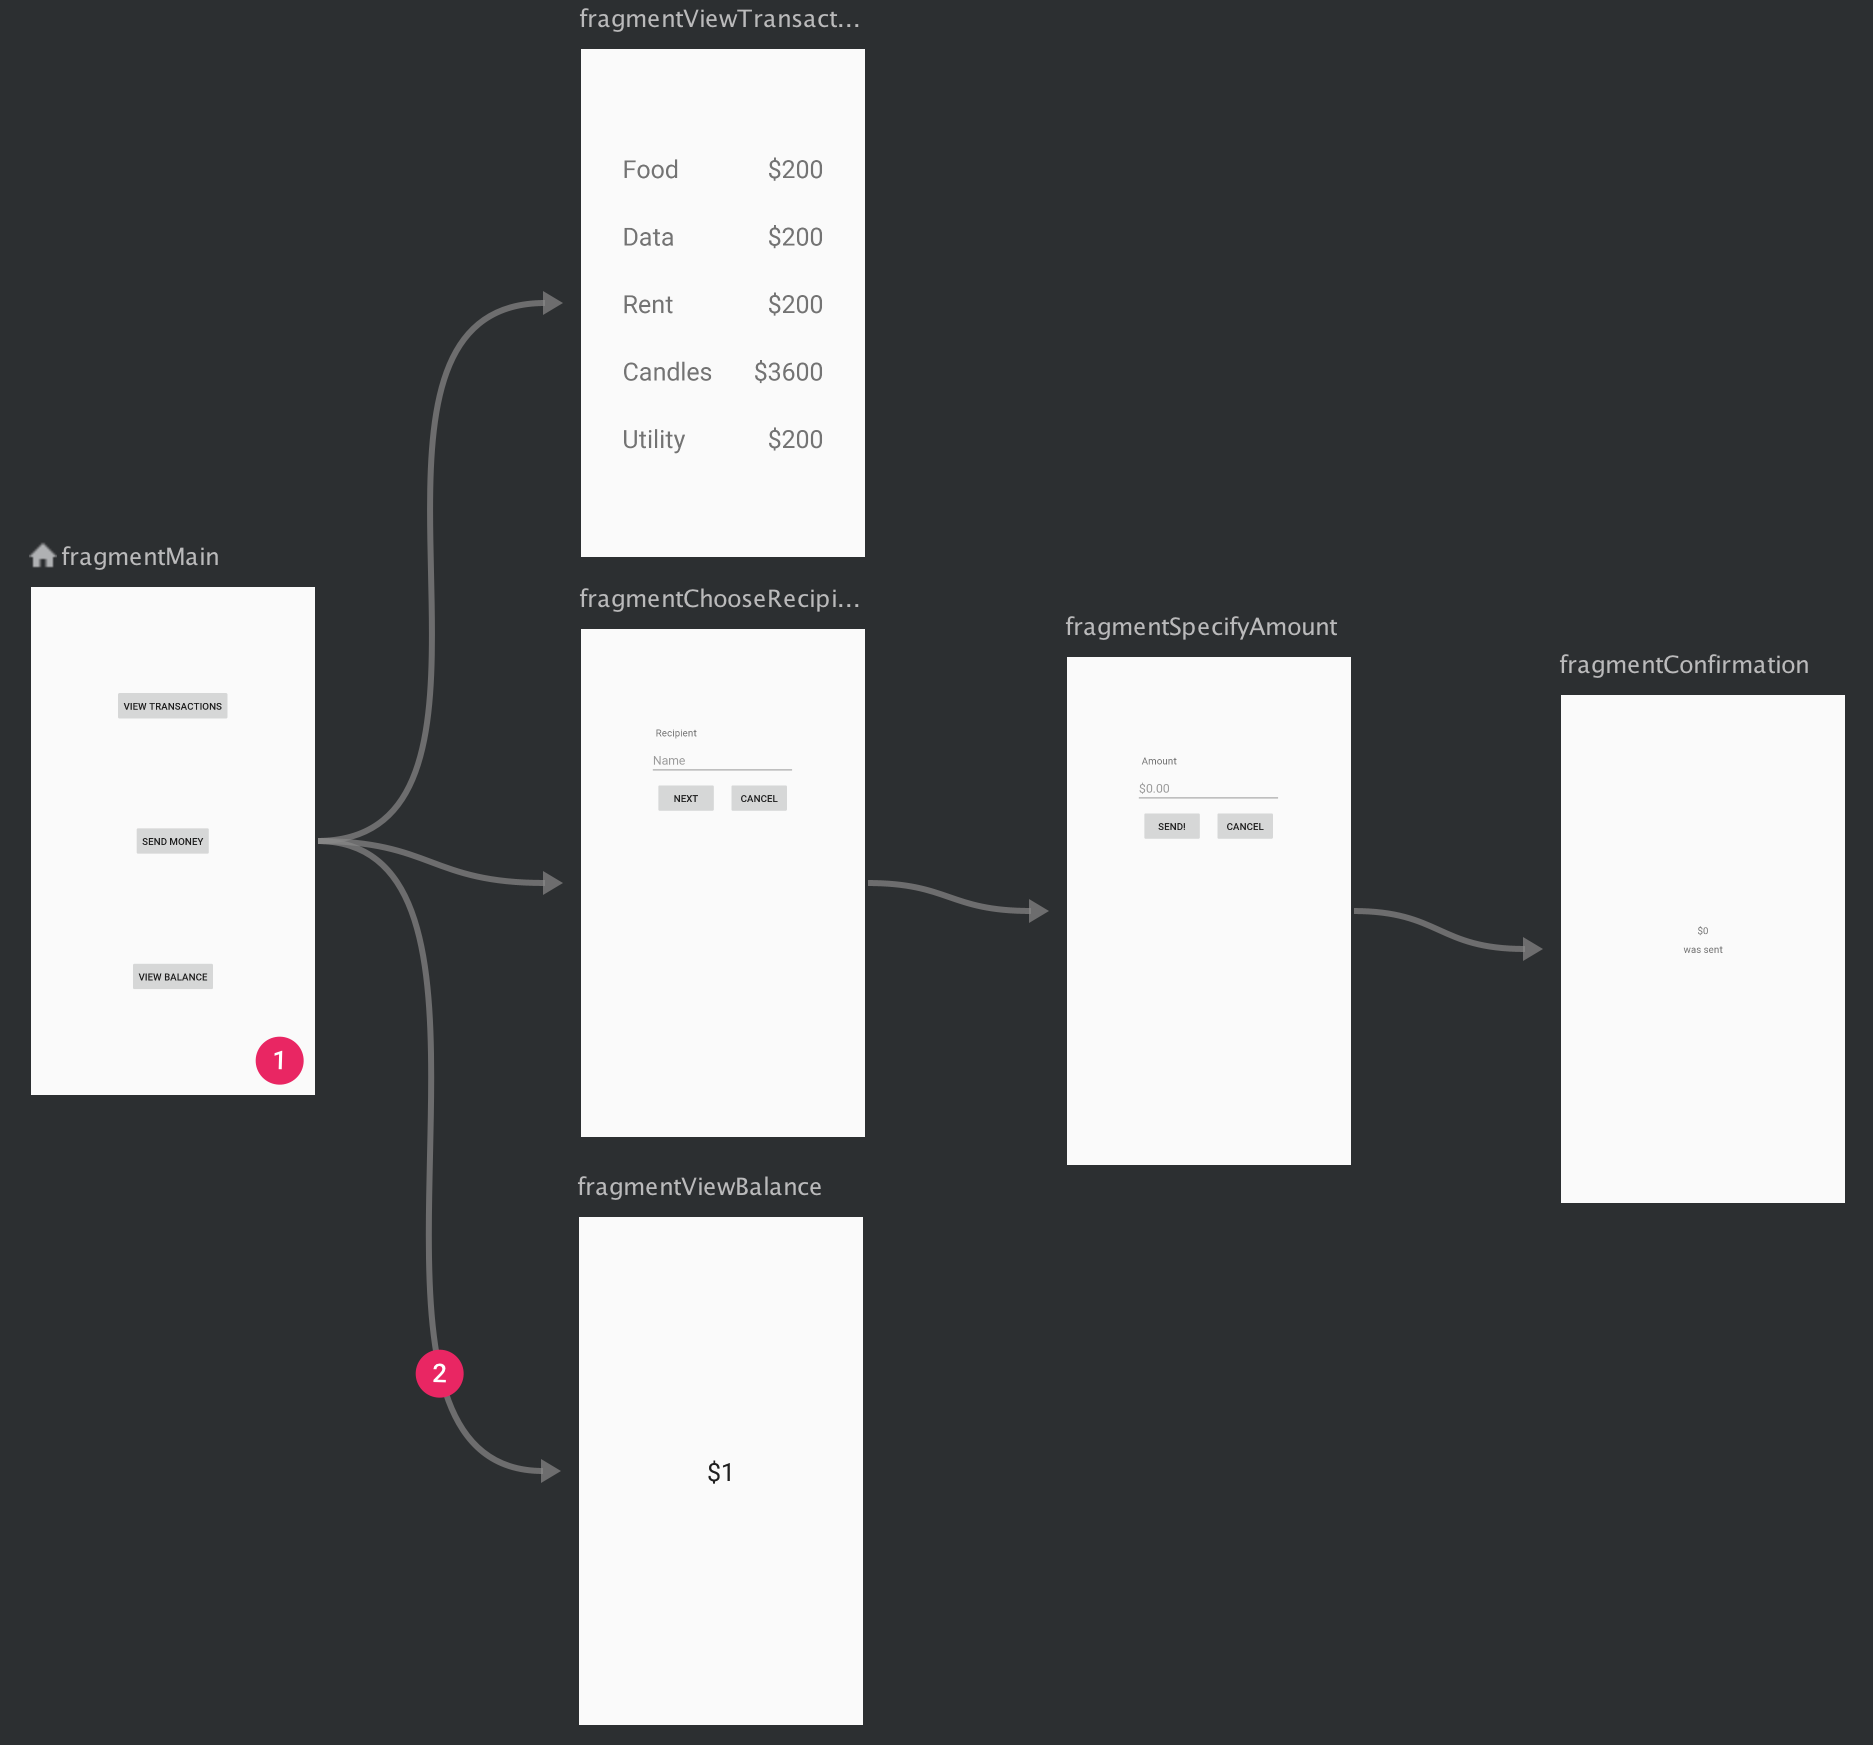
\includegraphics[width=0.45\textwidth]{navigation_graph.png}
\caption{\label{fig:nav_graph} Navigation Graph}
\end{figure}

\end{frame}

\section{Editor de navegación}

\begin{frame}{Como crear un gráfico?}

\begin{figure}
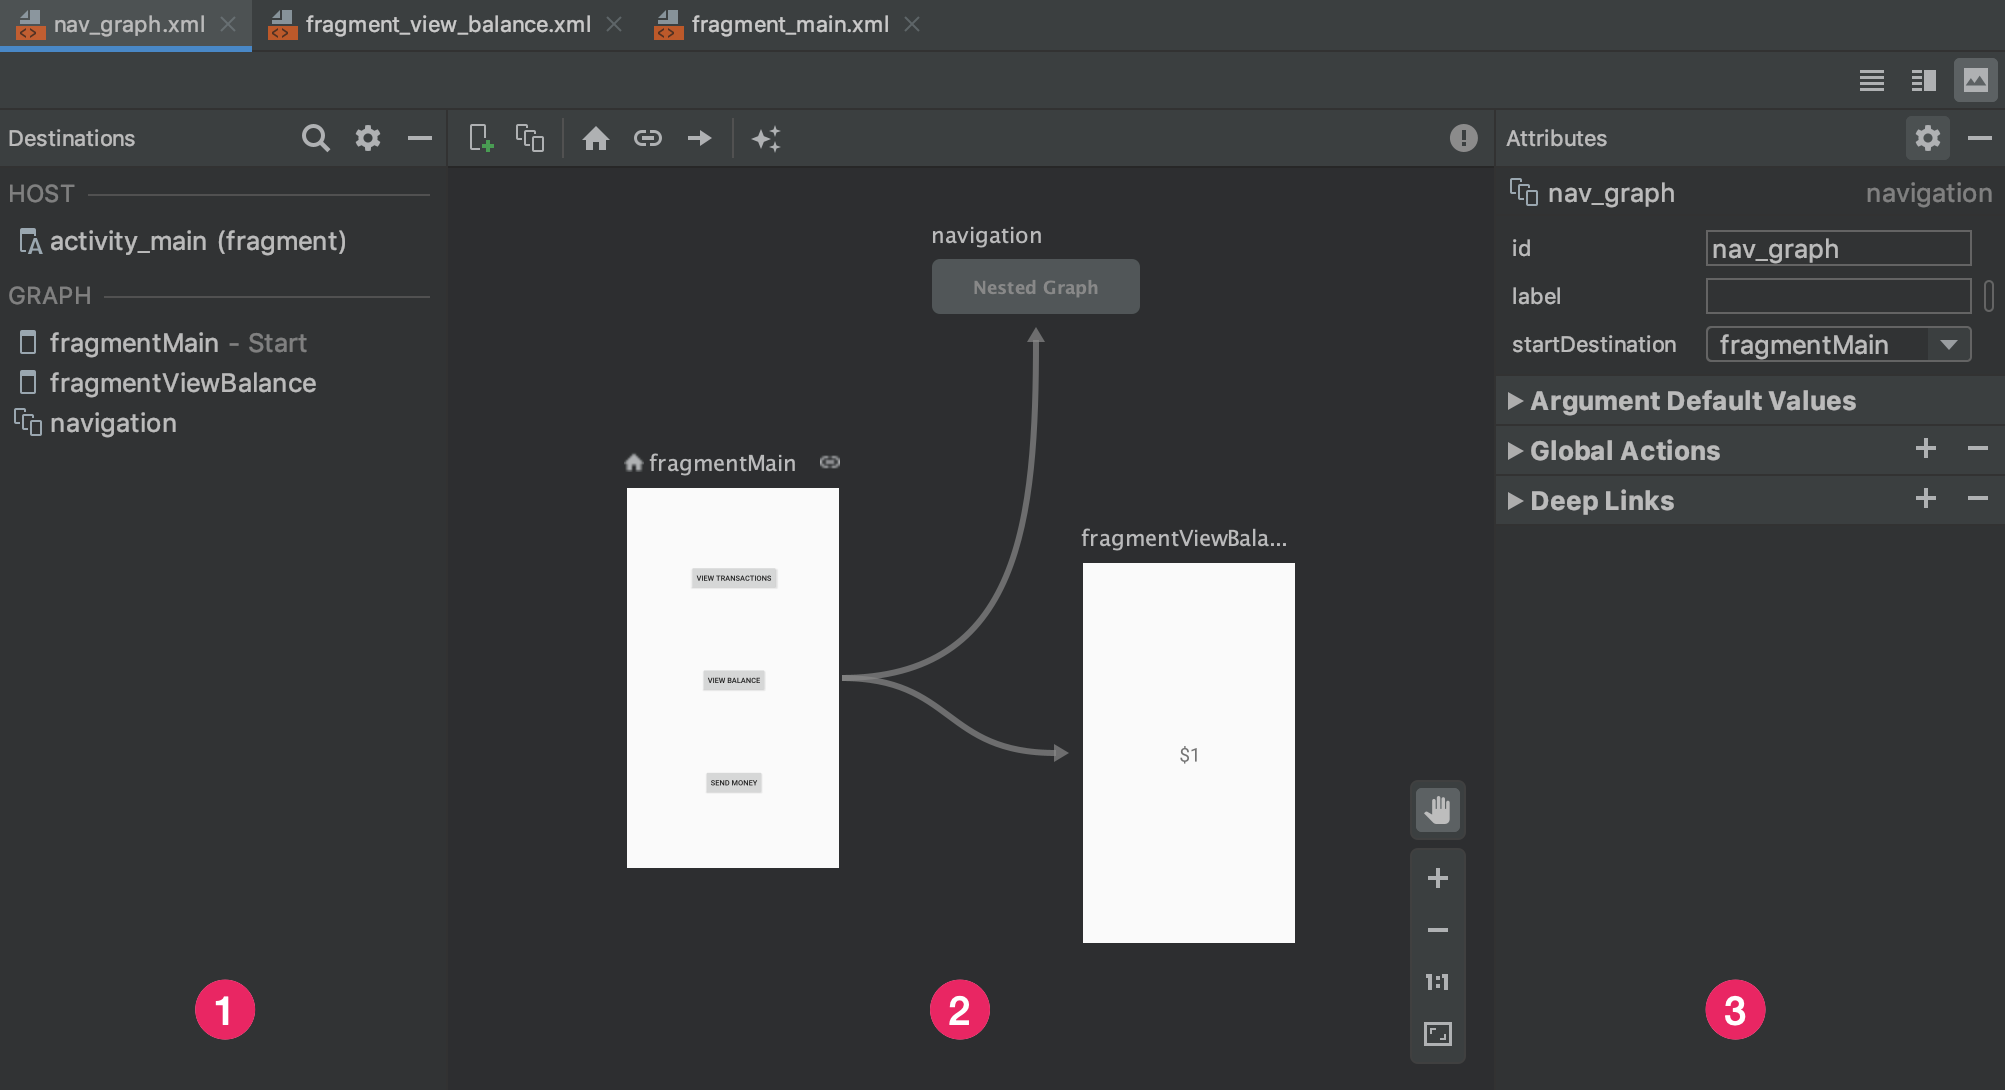
\includegraphics[width=0.75\textwidth]{nav-editor.png}
\caption{\label{fig:nav_graph} Editor de navegación}
\end{figure}

\end{frame}

\section{Que podemos hacer?}

\begin{frame}{Que podemos hacer con navigation component}

\justifying

\begin{itemize}
  \item Administrar transacciones de fragmentos.
  \item Administrar correctamente las acciones predeterminadas Arriba y Atrás.
  \item Proporcionar recursos estandarizados para animaciones y transiciones
  \item Safe Args, un complemento de Gradle que proporciona seguridad de tipo al navegar y pasar datos entre destinos
\end{itemize}

\end{frame}

\begin{frame}{Let do an example}

\begin{figure}
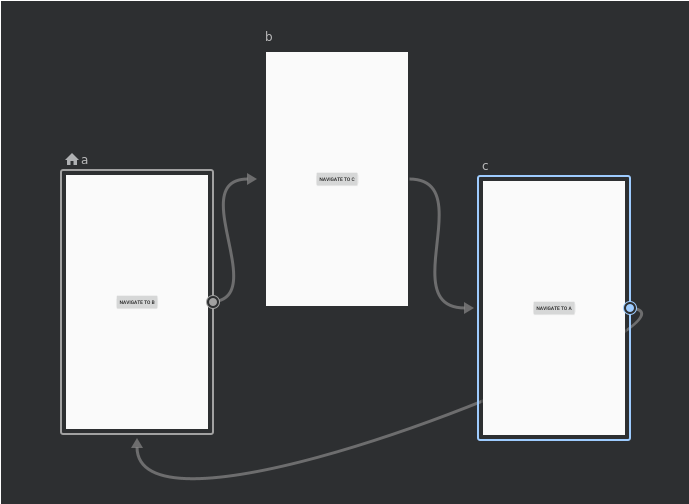
\includegraphics[width=0.6\textwidth]{work_flow.png}
\caption{Flujo a construir}
\end{figure}

\end{frame}

\begin{frame}{Referencias}

\justifying

\nocite{*}
\bibliographystyle{elsarticle-num} 
 \bibliography{ref}
\end{frame}

\end{document}
